\documentclass[10pt]{article}
\usepackage{icmlko}

\icmlmeta{IP 파운데이션 월드모델}{200}{보간으로 재고 외삽을 시켰다}{격차를 재는 마지막 방법 --- 접힘 교차로 학습 전체를 쓴다. 자료는 네 배로 늘었는데 부호는 더 틀렸고, 까닭이 한 줄이다}

\begin{document}

\twocolumn[
\icmlheader

\begin{abstract}
노트 199가 ``격차의 \emph{부호}만 필요하다면 접힘 교차로 학습 전체를 쓸 수
있다''를 남겼다. 했다 --- 도메인마다 학습을 시간 블록 넷으로 나누고 한
블록을 빼며 나머지 셋으로 적합해 뺀 블록에서 ``혼자 대 풀링''을 견주고
넷을 평균한다. 평가에 쓰이는 행이 25\%에서 \textbf{100\%}가 된다.
\textbf{그런데 부호가 더 틀린다.} 웹툰의 격차가 두 토막 $-$0.016 · 세 토막
$+$0.017 · \textbf{접힘 $+$0.041} 로 갈수록 나빠지고, 참값은 $-$0.158
(풀링이 훨씬 낫다)이다. 유보 곡선이 \textbf{완전 단조 감소}다(스피어만
$-$1.000) --- $k$ 를 키울수록 $+$0.3852 에서 $+$0.3521 로 떨어진다.
\textbf{까닭이 한 줄이다} --- 한 블록을 빼고 나머지 셋으로 적합하면 뺀
블록의 \emph{앞뒤가 다} 학습에 들어간다. 혼자 모형이 \textbf{보간} 문제를
푸는 것이다. 실제 과제는 2025년 이후를 맞히는 \textbf{외삽}이고, 보간에서
잘하는 모형이 외삽에서 잘한다는 보장이 없다 --- 노트 182가 잰 대로 웹툰은
축과 라벨의 관계가 시간에 시들기 때문에 특히 그렇다. \textbf{부호 정확도를
개수로 세면 안 갈린다} --- 두 토막 4/7 · 세 토막 4/7 · 접힘 3/7 이다.
\textbf{틀렸을 때 잃는 양으로 무게를 실으면 갈린다} --- \textbf{95.2\% ·
36.8\% · 34.7\%}. 웹툰 하나가 무게의 60\%이고 두 토막만 그것을 맞힌다.
\textbf{그래서 이 갈래(노트 197$\sim$200)의 답은 노트 197의 이분 규칙
하나다}($+$0.3955). 이제 왜 그것만 살아남았는지 안다 --- \textbf{앞으로만
보는 두 토막이 유일하게 부호를 맞히고, 이분이 크기를 안 쓰기 때문이다.}
\end{abstract}
]

\begin{figure*}[t]
\centering
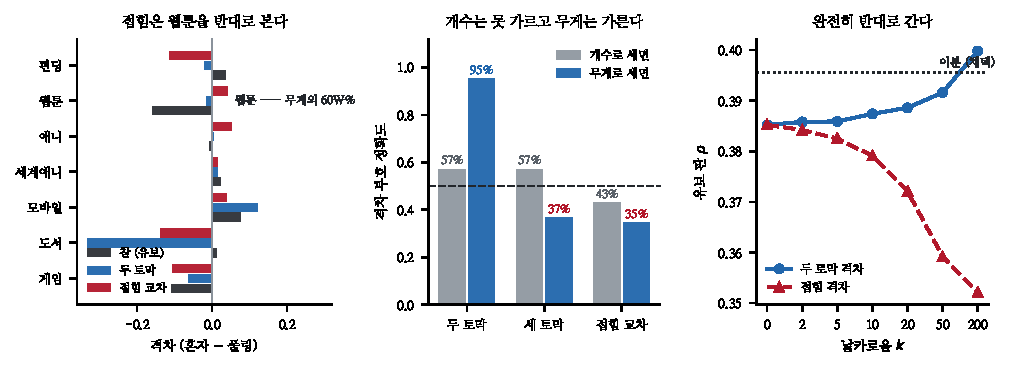
\includegraphics[width=\textwidth]{figs/interp.pdf}
\caption{왼쪽 --- 접힘은 웹툰을 반대로 본다. 가운데 --- 개수는 못 가르고
무게는 가른다. 오른쪽 --- 완전히 반대로 간다.}
\end{figure*}

\section{자료를 네 배 쓰고 더 틀렸다}

\begin{table}[t]
\centering\tsize
\caption{격차 추정 셋. 참값은 유보에서 잰 것.}
\begin{tabular}{lrrrr}
\toprule
& 참 & 두 토막 & 세 토막 & 접힘 \\
\midrule
\textbf{웹툰} & \textbf{$-$.158} & \textbf{$-$.016} & $+$.017 & \textbf{$+$.041} \\
게임 & $-$.108 & $-$.064 & $-$.302 & $-$.105 \\
모바일 & $+$.076 & $+$.123 & $+$.168 & $+$.039 \\
펀딩 & $+$.035 & $-$.021 & $-$.146 & $-$.115 \\
세계애니 & $+$.022 & $+$.014 & $+$.032 & $+$.015 \\
도서 & $+$.013 & $-$.332 & $-$.244 & $-$.137 \\
애니 & $-$.007 & $+$.003 & $-$.019 & $+$.052 \\
\bottomrule
\end{tabular}
\end{table}

\claimx{\textbf{평가 행이 25\%에서 100\%가 됐는데 웹툰이 더 틀린다}
($-$0.016 $\to$ $+$0.041). 자료를 늘린 것이 해가 됐다.}{그리고 유보 곡선이
완전 단조 감소다($\rho{=}-1.000$) --- 이 격차를 믿을수록 판이 내려간다.}

\section{까닭은 한 줄이다}

\claimx{\textbf{한 블록을 빼고 나머지 셋으로 적합하면 뺀 블록의 앞뒤가 다
학습에 들어간다.} 혼자 모형이 \emph{보간} 문제를 푼다.}{실제 과제는 2025년
이후를 맞히는 \emph{외삽}이다. 노트 182 가 웹툰의
\texttt{goods\_scale} 이 학습 $+$0.378 에서 유보 $-$0.283 으로 뒤집히는
것을 쟀는데, \textbf{보간에서는 그 뒤집힘이 안 보인다} --- 양쪽에서 끼워
맞추면 되기 때문이다.}

\claimx{\textbf{그래서 웹툰에서 제일 크게 틀린다.} 웹툰이 시간 이동이
제일 심한 도메인이고(노트 182의 자기 전이 $+$0.037), 보간이 그 이동을
가려 준다.}{게임 · 세계애니처럼 관계가 안정된 도메인은 접힘이 참값에 제일
가깝다($-$0.105 대 참 $-$0.108, $+$0.015 대 $+$0.022). \textbf{접힘이
나쁜 것이 아니라 시간이 움직이는 도메인에서 나쁘다.}}

\section{개수로 세면 안 갈린다}

\begin{table}[t]
\centering\tsize
\caption{격차 부호 정확도.}
\begin{tabular}{lrr}
\toprule
& 개수 & \textbf{무게} \\
\midrule
\textbf{앞으로 두 토막} & 4/7 & \textbf{95.2\%} \\
앞으로 세 토막 & 4/7 & 36.8\% \\
접힘 교차 & 3/7 & 34.7\% \\
\bottomrule
\end{tabular}
\end{table}

\claimx{\textbf{개수로는 셋이 다 비슷한데}(4/7 · 4/7 · 3/7) \textbf{무게를
실으면 95\% 대 37\% 대 35\%다.} 무게는 유보 표본 $\times$ $|$참 격차$|$ ---
틀렸을 때 실제로 잃는 판 몫이다.}{웹툰 하나가 무게의 \textbf{60\%}이고
두 토막만 그것을 맞힌다. 나머지 여섯은 다 합쳐 40\%다.}

\claimx{\textbf{규약으로 적는다: 부호 정확도를 개수로 세지 말 것.} 셀 때
쓰는 무게는 그 부호를 틀렸을 때 잃는 양이어야 한다.}{노트 183의 그늘이
``판이 크기 가중이라 작은 도메인을 숨긴다''를 잡았는데, 여기는 반대다 ---
\textbf{개수로 세면 큰 도메인이 숨는다.}}

\section{갈래를 닫는다}

\begin{table}[t]
\centering\tsize
\caption{노트 197$\sim$200. 도메인별 풀링을 정하는 네 방법.}
\begin{tabular}{lrl}
\toprule
& 판 $\rho$ & \\
\midrule
완전 분리 & .3445 & \\
완전 풀링 & .3822 & \\
\textbf{이분 (노트 197)} & \textbf{.3955} & \textbf{채택} \\
축소 비율 · 두 토막 & .3886 & 규약이 막음 \\
축소 비율 · 세 토막 & .3852 & 규약이 막음 \\
축소 비율 · 접힘 & .3852 & $k{=}0$ 이 최선 \\
\bottomrule
\end{tabular}
\end{table}

\claimx{\textbf{이제 왜 이분만 살아남았는지 안다.} 앞으로만 보는 두 토막이
유일하게 부호를 맞히고(무게 95\%), 이분은 그 부호만 쓰고 크기를 안
쓴다.}{노트 198이 ``잡음이 크기에 있고 신호가 부호에 있다''를 적었고, 노트
200이 ``그 부호를 맞히는 추정기가 하나뿐''임을 더한다. \textbf{두 사실이
합쳐져 이분 규칙을 설명한다.}}

\claimx{\textbf{이 갈래의 총 이득은 $+$0.0133 이다}(완전 풀링 $+$0.3822
$\to$ 이분 $+$0.3955). 그중 모바일 한 도메인이 93\%다.}{그리고 능형이
$+$0.3709(노트 194 전)에서 여기까지 오는 동안 챔피언과의 격차가 0.078
에서 0.053 으로 줄었다 --- 다만 이 갈래는 최근 가중과 아직 합치지
않았다.}

\begin{table}[t]
\centering\tsize
\caption{남은 것.}
\begin{tabular}{ll}
\toprule
\textbf{합치기} & 최근 가중($\tau{=}2$)과 도메인별 풀링을 함께 \\
트리 & 이 갈래 넷이 전부 능형만 \\
웹툰 & 접힘이 왜 그 도메인만 크게 틀리나 --- 쟀다 \\
\bottomrule
\end{tabular}
\end{table}

첫 줄이 곧바로 할 수 있고 값이 크다. 최근 가중이 $+$0.0304 였고 도메인별
풀링이 $+$0.0133 인데 \textbf{둘을 합치면 얼마인지 안 쟀다.} 겹칠 이유가
있다 --- 최근 가중은 옛 행을 덜 믿는 것이고 도메인별 풀링은 남의 행을 덜
믿는 것이라, 둘 다 ``웹툰의 옛 자료''를 겨냥한다. \textbf{겹치면 $+$0.03
에 그치고 안 겹치면 $+$0.044 다.} 노트 195에서 $\tau$ 와 $\alpha$ 를 같이
고르면 나빠졌으니 이번에도 순차로 해야 한다.

\end{document}
